\documentclass[german]{cgspaper} % change option to 'english' to include english logo in \copyrightspace

\usepackage[ngerman]{babel} % comment out to use english in auto-generated section titles
\usepackage[utf8]{inputenc}
\usepackage[ruled]{algorithm}
\usepackage{algpseudocode}
\usepackage{url}
\usepackage{color}

\definecolor{colorMartin}{RGB}{147,83,177}
\definecolor{colorPascal}{RGB}{255,127,0}
\definecolor{colorTobias}{RGB}{160,123,46}

\newcommand{\Martin}[1]{ \textcolor{colorMartin}{TODO Martin:} #1 }
\newcommand{\Pascal}[1]{ \textcolor{colorPascal}{TODO Pascal:} #1 }
\newcommand{\Tobias}[1]{ \textcolor{colorTobias}{TODO Tobias:} #1 }

\newcommand{\neuerBegriff}[1]{\textit{#1}}

\title{Selfaware Monopoly}
\author{John Doe\\ Digital Engineering Fakultät, Hasso-Plattner-Institut \textbar{} Universität Potsdam}

% Konfiguration des Veranstaltungs-Feldes
\subject{%
    \textbf{Advanced Games of Life}\\
    Sommersemester 2018\\
    Themenstellung und Anleitung:
    XX und Prof.\ Dr.\ Jürgen Döllner}

\begin{document}

% Definition des Teasers
\teaser{
    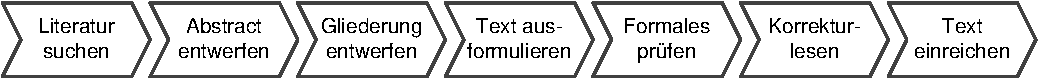
\includegraphics[width=0.9\textwidth]{graphics/prozess.pdf}
    \caption{Beispiel für einen Teaser: Schritte beim Erstellen eines fachwissenschaftlichen Beitrags. Ein Teaser dient als Blickfang schon auf der ersten Seite eines Artikels.}
    \label{fig:prozess}
}

\maketitle

%----------------------------------------------------------------
% Zusammenfassung
%----------------------------------------------------------------
\begin{abstract}
\end{abstract}

\copyrightspace % Erzeugt den Hinweis auf die Veranstaltung links unten

\section{Aufgabenstellung}
Inhaltlich erwarten wir die wissenschaftliche Auseinandersetzung mit dem bearbeiteten Seminarthema. Analog zum Abschlussvortrag empfehlen wir eine Einführung in das Thema, die Vorstellung des technischen Prototypen (Architektur, Designentscheidungen, Umsetzung), eine Diskussion über Relevanz des bearbeiteten Themas in der Gesellschaft und Vorstellen von Eigenschaften und Ergebnissen eures Prototyps. Die Struktur der Ausarbeitung und genaue Themen besprecht ihr am Besten mit eurem Betreuer.

%----------------------------------------------------------------
% Einleitung
%----------------------------------------------------------------
\section{Einleitung}

Informations Systeme ersetzen immer mehr elementare Bestandteile unserer Gesellschaft.
Soziale Netzwerke, das Finanz- und Bankwesen, Wahlsysteme um nur eine wenige Bereiche zu nennen.
Dabei Vertrauen alle Beteiligten darauf das diese Systeme sich an die Regeln halten und alle Beteiligeten gleichermaßen fair behandeln.

Was wäre wenn dies nicht der Fall ist? 
Was wäre wenn innerhalb des Systems Hintertüren existieren, welche es ermöglichen einzelne Regeln zu umgehen.
Was wäre wenn das System durch das benutzen dieser Hintertüren, die Grenzen seiner Spezifikation überschreitet und sich so Zugang zu Information und Ressourcen verschafft, welche es nicht besitzen dürfte.

Im Rahmen des Seminars Games of Life wollen wir ein solches System konzipieren und implementieren.

\section{Konzept}

Das Spiel Monopoly war urpsrünglich als Gesellschaftskritik am Kapitalismus gedacht. \Martin{Nachweis} 
Aufbauend auf dieser Grundidee wollen wir nun ein Spiel entwerfen, welches dem Spieler die Möglichkeit gibt die Spielregeln zu umgehen und sich im Gegenzug Information und Resourcen vom Spieler beschaft. 
Diese Komponente wird im folgenden \neuerBegriff{Watson} genannt.

\subsection{Watson}

Watson bietet den Spieler immer wieder die Möglichkeit, die Regel von Monopoly zu umgehen und dem Spieler so einen Vorteil zu verschaffen.
Die Spieler müssen dafür aber aktiv die Entscheidung treffen, dass sie Watson nutzen.
Im Gegenzug wird Watson versuchen unterschiedliche Ressourcen die nicht Inhalt des Spiels sind vom Spieler zu erhalten.
Dazu zählen persöhliche Information, wie zum Beispiel die Identität des Spielers auf Facebook, Twitter oder anderen Sozialen Platformen, Rechnenleistung um zum Beispiel Bitcoinmining zu betreiben oder im Namen anderer Aktionen wie Likes, Reviews oder Kommentare zu erstellen.

\subsubsection{Was will Watson?}

\Martin{Informationsraub beschreiben}

\Pascal{Welche APIs}

\subsubsection{Was bietet Watson den Spielern}

\Martin{Schummelmatrix beschreiben}

\section{Vorstellung Prototyp}

\Tobias{Architektur, Designentscheidungen, Umsetzung}
\Tobias{Eigenschaften und Ergebnisse beschreiben}

\Pascal{Apis beschreiben}

\section{Diskussion}

\subsection{Apis}

\Pascal{Was könnten man als Insider in mit den Apis tun?}

\subsection{Relevanz innerhalb der Gesselschaft}

\Martin{Relevanz beschreiben}



\bibliographystyle{acmsiggraph}
\bibliography{gol-selfaware-monopoly}

\end{document}
